%!TEX program = lualatex
% img.tex
\documentclass{article}

\usepackage{emoji}
\usepackage{graphicx}
\usepackage{float}
\usepackage{subfig}

% custom path
\graphicspath{img/}

\title{Image \emoji{book}}
\author{oeyoews}
\date{2022/08/09}

\begin{document}

\maketitle

% \listoffigures

\section{Images \emoji{book}}
\label{sec:img}

\begin{figure}[H]
	\centering
	% not support subfile for prefix
	
\includegraphics[width=0.7\textwidth]{img/01.png}
	\caption{Fig01}
	\label{Fig01}
	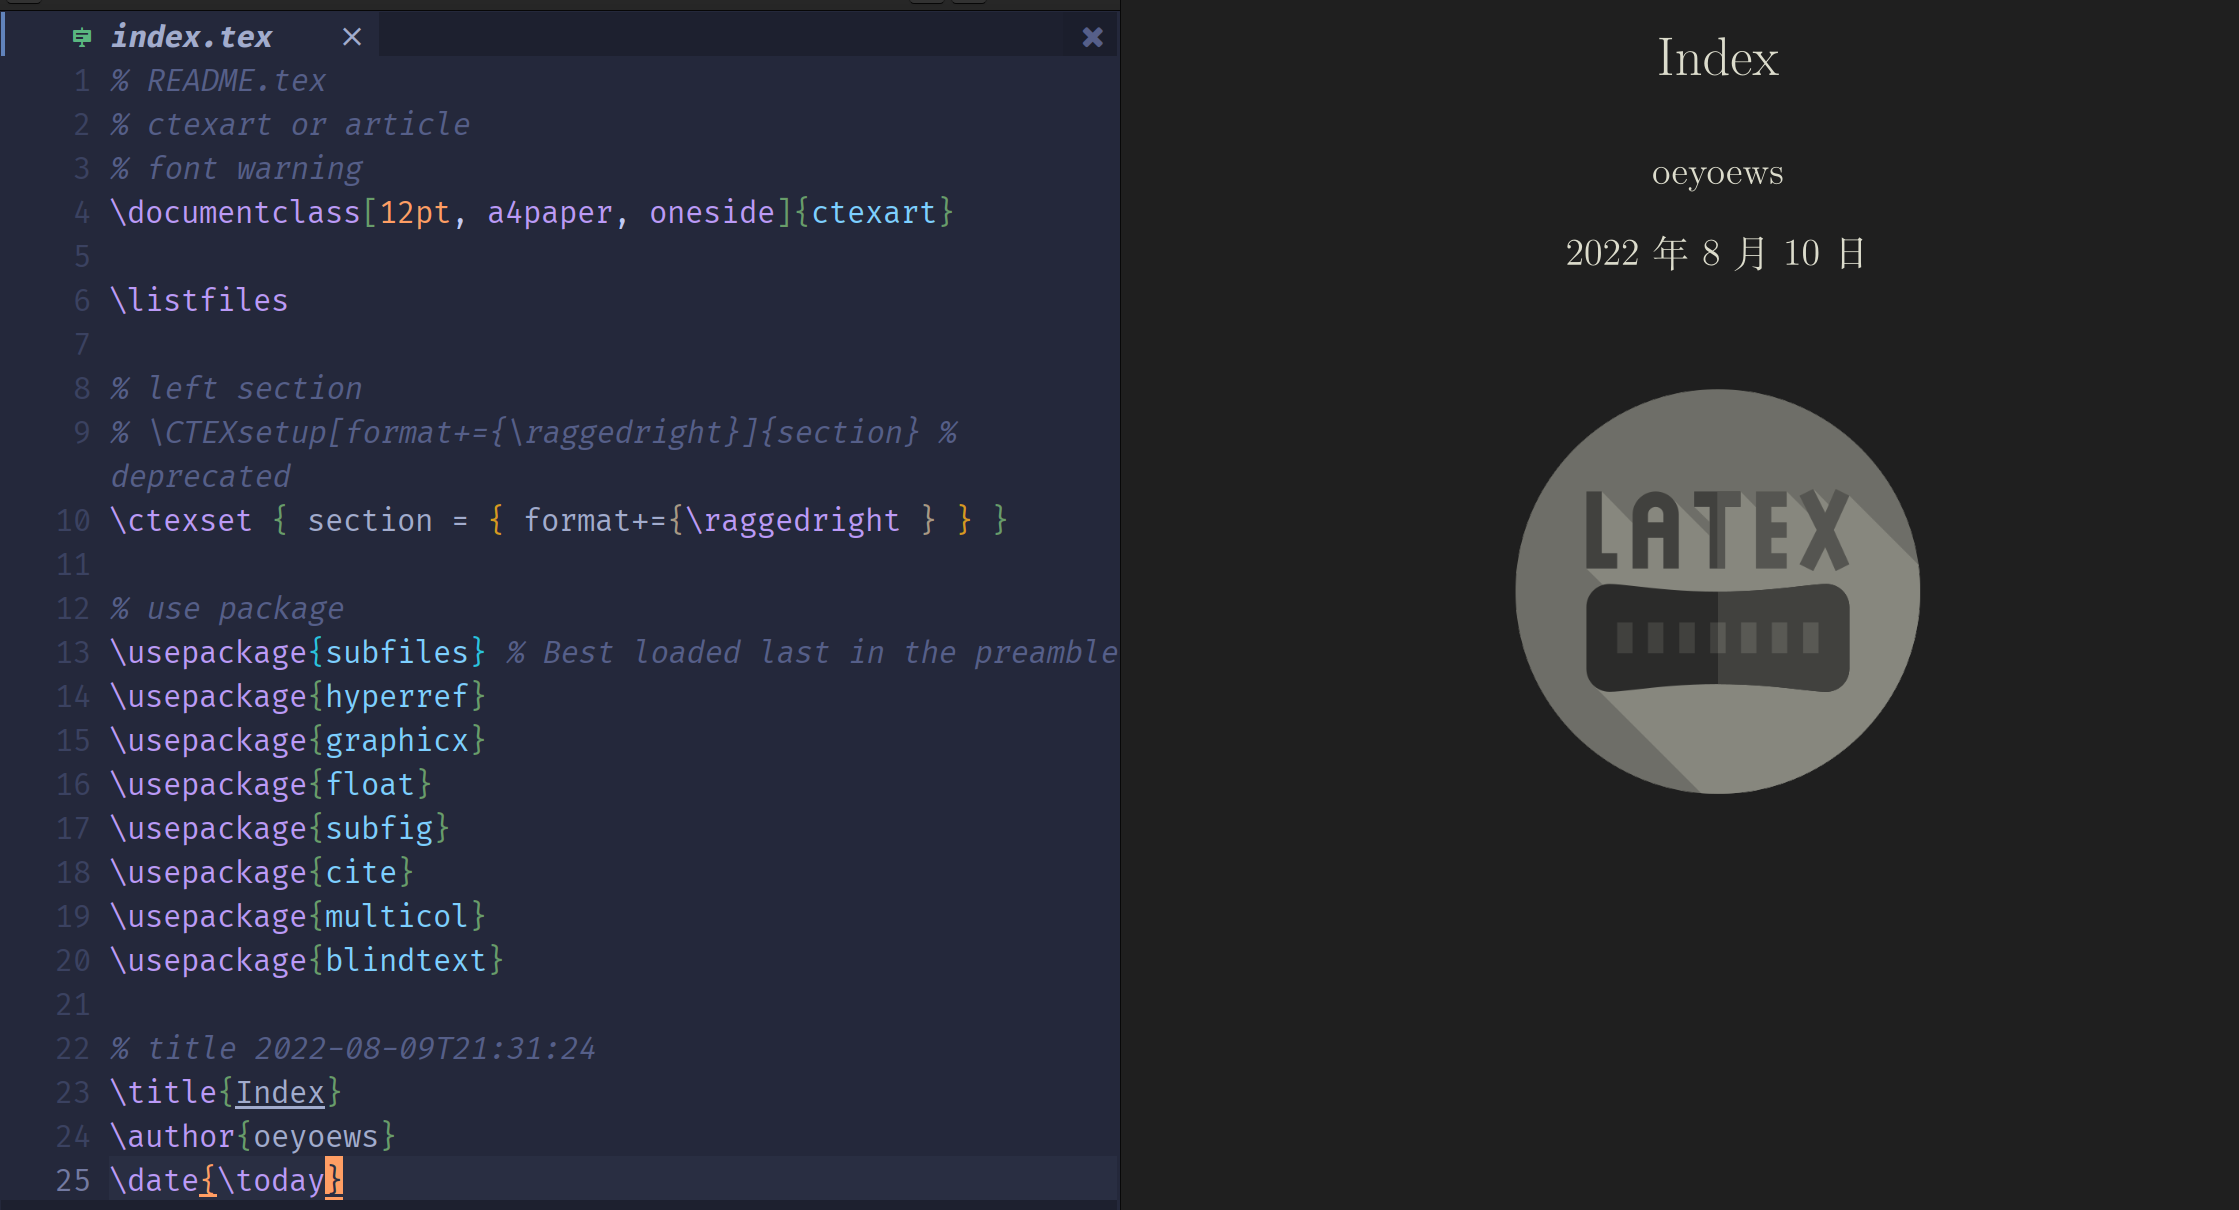
\includegraphics[width=0.7\textwidth]{img/02.png}
	\caption{Fig02}
	\label{Fig02}
\end{figure}

\end{document}
